%%%%%%%%%%%%%%%%%%%%%%%%%%%%%%%%%%%%%%%%%
% Masters/Doctoral Thesis 
% LaTeX Template
% Version 2.5 (27/8/17)
%
% This template was downloaded from:
% http://www.LaTeXTemplates.com
%
% Version 2.x major modifications by:
% Vel (vel@latextemplates.com)
%
% This template is based on a template by:
% Steve Gunn (http://users.ecs.soton.ac.uk/srg/softwaretools/document/templates/)
% Sunil Patel (http://www.sunilpatel.co.uk/thesis-template/)
%
% Template license:
% CC BY-NC-SA 3.0 (http://creativecommons.org/licenses/by-nc-sa/3.0/)
%
%%%%%%%%%%%%%%%%%%%%%%%%%%%%%%%%%%%%%%%%%

%----------------------------------------------------------------------------------------
%	PACKAGES AND OTHER DOCUMENT CONFIGURATIONS
%----------------------------------------------------------------------------------------

\documentclass[
11pt, % The default document font size, options: 10pt, 11pt, 12pt
%oneside, % Two side (alternating margins) for binding by default, uncomment to switch to one side
english, % ngerman for German
singlespacing, % Single line spacing, alternatives: onehalfspacing or doublespacing
%draft, % Uncomment to enable draft mode (no pictures, no links, overfull hboxes indicated)
%nolistspacing, % If the document is onehalfspacing or doublespacing, uncomment this to set spacing in lists to single
%liststotoc, % Uncomment to add the list of figures/tables/etc to the table of contents
%toctotoc, % Uncomment to add the main table of contents to the table of contents
%parskip, % Uncomment to add space between paragraphs
%nohyperref, % Uncomment to not load the hyperref package
headsepline, % Uncomment to get a line under the header
%chapterinoneline, % Uncomment to place the chapter title next to the number on one line
%consistentlayout, % Uncomment to change the layout of the declaration, abstract and acknowledgements pages to match the default layout
]{MastersDoctoralThesis} % The class file specifying the document structure
\documentclass{article}
\usepackage{ragged2e}
\usepackage[utf8]{inputenc} % Required for inputting international characters
\usepackage[T1]{fontenc} % Output font encoding for international characters

\usepackage{mathpazo} % Use the Palatino font by default

\usepackage[backend=bibtex,style=authoryear,natbib=true]{biblatex} % Use the bibtex backend with the authoryear citation style (which resembles APA)

\addbibresource{example.bib} % The filename of the bibliography

\usepackage[autostyle=true]{csquotes} % Required to generate language-dependent quotes in the bibliography

%----------------------------------------------------------------------------------------
%	MARGIN SETTINGS
%----------------------------------------------------------------------------------------

\geometry{
	paper=a4paper, % Change to letterpaper for US letter
	inner=2.5cm, % Inner margin
	outer=3.8cm, % Outer margin
	bindingoffset=.5cm, % Binding offset
	top=1.5cm, % Top margin
	bottom=1.5cm, % Bottom margin
	%showframe, % Uncomment to show how the type block is set on the page
}

%----------------------------------------------------------------------------------------
%	THESIS INFORMATION
%----------------------------------------------------------------------------------------

\thesistitle{Laptop Price Prediction using Machine Learning} % Your thesis title, this is used in the title and abstract, print it elsewhere with \ttitle
\supervisor{Dr. Muneendra \textsc{Ojha}} % Your supervisor's name, this is used in the title page, print it elsewhere with \supname
\examiner{} % Your examiner's name, this is not currently used anywhere in the template, print it elsewhere with \examname
\degree{Bachelor of Technology} % Your degree name, this is used in the title page and abstract, print it elsewhere with \degreename
\author{Hritik \textsc{Kumar}} % Your name, this is used in the title page and abstract, print it elsewhere with \authorname
\addresses{} % Your address, this is not currently used anywhere in the template, print it elsewhere with \addressname

\subject{Machine Learning} % Your subject area, this is not currently used anywhere in the template, print it elsewhere with \subjectname
\keywords{} % Keywords for your thesis, this is not currently used anywhere in the template, print it elsewhere with \keywordnames
\university{\href{https://www.iiita.ac.in/}{Indian Institute of Information Technology, Allahabad}} % Your university's name and URL, this is used in the title page and abstract, print it elsewhere with \univname
\department{{Information Technology}} % Your department's name and URL, this is used in the title page and abstract, print it elsewhere with \deptname
%\group{\href{http://researchgroup.university.com}{Research Group Name}} % Your research group's name and URL, this is used in the title page, print it elsewhere with \groupname
\faculty{{Muneendra Ojha}} % Your faculty's name and URL, this is used in the title page and abstract, print it elsewhere with \facname

\AtBeginDocument{
\hypersetup{pdftitle=\ttitle} % Set the PDF's title to your title
\hypersetup{pdfauthor=\authorname} % Set the PDF's author to your name
\hypersetup{pdfkeywords=\keywordnames} % Set the PDF's keywords to your keywords
}

\begin{document}

\frontmatter % Use roman page numbering style (i, ii, iii, iv...) for the pre-content pages

\pagestyle{plain} % Default to the plain heading style until the thesis style is called for the body content

%----------------------------------------------------------------------------------------
%	TITLE PAGE
%----------------------------------------------------------------------------------------

\begin{titlepage}
\begin{center}

\vspace*{.06\textheight}
{\scshape\LARGE \univname\par}\vspace{1.5cm} % University name
\textsc{\Large Project Report}\\[0.5cm] % Thesis type

\HRule \\[0.4cm] % Horizontal line
{\huge \bfseries \ttitle\par}\vspace{0.4cm} % Thesis title
\HRule \\[1.5cm] % Horizontal line
 
\begin{minipage}[t]{0.4\textwidth}
\begin{flushleft} \large
\emph{Author:}\\
{\authorname} % Author name - remove the \href bracket to remove the link
\end{flushleft}
\end{minipage}
\begin{minipage}[t]{0.4\textwidth}
\begin{flushright} \large
\emph{Supervisor:} \\
{\supname} % Supervisor name - remove the \href bracket to remove the link  
\end{flushright}
\hspace{-2.0cm}
\includegraphics[scale=0.5]{download.png}
\end{minipage}\\[3cm]
 
\vfill

\large \textit{A thesis submitted in fulfillment of the requirements\\ for the degree of \degreename}\\[0.3cm] % University requirement text
\textit{in the}\\[0.4cm]
\deptname\\[2cm] % Research group name and department name
 
\vfill

{\large \today}\\[4cm] % Date
% 
\includegraphics[scale=0.5]{download.png} % University/department logo - uncomment to place it
 
\vfill
\end{center}
\end{titlepage}
% {
\includegraphics[scale=0.5]{download.png}}

%----------------------------------------------------------------------------------------
%	DECLARATION PAGE
%----------------------------------------------------------------------------------------

% \begin{declaration}
% \addchaptertocentry{\authorshipname} % Add the declaration to the table of contents
% \noindent I, \authorname, declare that this thesis titled, \enquote{\ttitle} and the work presented in it are my own. I confirm that:

% \begin{itemize} 
% \item This work was done wholly or mainly while in candidature for a research degree at this University.
% \item Where any part of this thesis has previously been submitted for a degree or any other qualification at this University or any other institution, this has been clearly stated.
% \item Where I have consulted the published work of others, this is always clearly attributed.
% \item Where I have quoted from the work of others, the source is always given. With the exception of such quotations, this thesis is entirely my own work.
% \item I have acknowledged all main sources of help.
% \item Where the thesis is based on work done by myself jointly with others, I have made clear exactly what was done by others and what I have contributed myself.\\
% \end{itemize}
 
% \noindent Signed:\\
% \rule[0.5em]{25em}{0.5pt} % This prints a line for the signature
 
% \noindent Date:\\
% \rule[0.5em]{25em}{0.5pt} % This prints a line to write the date
% \end{declaration}

% \cleardoublepage

%----------------------------------------------------------------------------------------
%	QUOTATION PAGE
%----------------------------------------------------------------------------------------

% \vspace*{0.2\textheight}

% \noindent\enquote{\itshape Thanks to my solid academic training, today I can write hundreds of words on virtually any topic without possessing a shred of information, which is how I got a good job in journalism.}\bigbreak

% \hfill Dave Barry

%----------------------------------------------------------------------------------------
%	ABSTRACT PAGE
%----------------------------------------------------------------------------------------

\begin{abstract}
\addchaptertocentry{\abstractname} % Add the abstract to the table of contents
This paper presents a Laptop price prediction system by using the supervised machine learning 
technique. The research uses multiple linear regression as the machine learning prediction method which 
offered 81 percent prediction precision. Using multiple linear regression, there are multiple independent variables 
but one and only one dependent variable whose actual and predicted values are compared to find precision of 
results. This paper proposes a system where price is dependent variable which is predicted, and this price is 
derived from factors like Laptop’s model, RAM, ROM (HDD/SSD), GPU, CPU, IPS Display, and Touch 
Screen. Since the COVID-19 pandemic, many activities are now carried out in a Work From Home 
(WFH) manner. According to data from the Central Statistics Agency (BPS) of East Java, in 2021, large and 
medium-sized enterprises (UMB) who choose to work WFH partially are 32.37 percent, and overall WFH is 2.24 percent 
(BPS East Java, 2021 ). With this percentage of 32.37 percent, many people need a work device (in this case, a laptop) 
that can boost their productivity during WFH. WFH players must have laptops with specifications that match 
their needs to encourage productivity. To prevent buying laptops at overpriced prices, a way to predict laptop 
prices is needed based on the specified specifications. This study presents a Machine Learning model from data 
acquisition (Data Acquisition), Data Cleaning, and Feature Engineering for the Pre-Processing, Exploratory Data 
Analysis stages to modeling based on regression algorithms.
\ldots
\end{abstract}

%----------------------------------------------------------------------------------------
%	ACKNOWLEDGEMENTS
%----------------------------------------------------------------------------------------

% \begin{acknowledgements}
% \addchaptertocentry{\acknowledgementname} % Add the acknowledgements to the table of contents
% The acknowledgments and the people to thank go here, don't forget to include your project advisor\ldots
% \end{acknowledgements}

%----------------------------------------------------------------------------------------
%	LIST OF CONTENTS/FIGURES/TABLES PAGES
%----------------------------------------------------------------------------------------

% \begin{document}

\tableofcontents % This command generates the table of contents

\chapter{Literature Review}
% Content for Literature Review section goes here
The literature review for laptop price prediction focuses on using machine learning techniques to forecast the cost of laptops. Multiple linear regression is commonly used as a prediction method, with factors such as laptop model, RAM, ROM, GPU, CPU, IPS display, and touch screen being considered as independent variables. Studies have also employed support vector regression, decision tree regression, and multi-linear regression to accurately predict laptop prices. Machine learning models like decision trees, multiple linear regression, KNN, and random forest have been tested to determine the most accurate prediction model. The aim is to assist buyers in making purchasing decisions by providing accurate price predictions based on real-time data scraped from e-commerce websites.\hfill\break\break
[1]. Sorower MS, published the paper (A literature survey on algorithms for multi-label learning). Various studies have extensively researched predicting 
the lifetime of laptops. In her Master's thesis, Listian found that using a regression model built with Decision Tree and Random Forest Regressor provided 
more precise predictions for the price of a leased laptop compared to using multivariate regression or simple multiple regression. This is because the 
Decision Tree Algorithm is more efficient in handling datasets with higher dimensions and is less susceptible to overfitting and underfitting. However, 
the weakness of this research lies in the lack of comparison between the basic indicators such as mean, variance, or standard deviation of simple regression 
and the more advanced Decision Tree Algorithm regression. Additionally, the research focused solely on supervised learning algorithms, limiting the scope of predictions.\hfill\break\break
[2].Pandey M, Sharma VK, published the paper (A decision tree algorithm pertaining to the student performance analysis and prediction. To fully utilize 
a predictive analytics solution and make informed decisions based on data, it is important for a company to identify the most suitable predictive modeling techniques. Predictive analytics tools employ a variety of models and algorithms that can be applied across a wide range of use cases. Machine Learning 
is an AI application that utilizes algorithms to process or assist with statistical data processing. Although it incorporates automation concepts, it still 
necessitates human guidance.\hfill\break\break
[3]. Priyama A, Abhijeeta RG, Ratheeb A, Srivastavab S, published the paper (Comparative analysis of decision tree classification algorithms) In the past 
decade, researchers have been increasingly interested in predicting the lifetime of laptops. To detect fake and real news regarding job advertisements on 
social media, classifiers such as the support vector machine (SVM), XGBoost classifier, and random forest classifier (RF) have been extensively used. 
Distinguishing between fake and real news can be challenging due to subtle differences in topics and word embeddings, which can impact the accuracy 
of the system. To prepare job post data for analysis, preprocessing steps such as stop word removal, tokenization, and lemmatization of words are 
performed using WordNet. The oversampling procedure is utilized to balance the data. Subsequently, new columns representing each possible attribute 
value from the original data are generated through one-hot encoding. Removal of insignificant features in the dataset is performed to facilitate laptop 
lifetime detection.\hfill\break\break
[4]. Noor, K., and Jan, S. published the paper (Laptop lifetime Prediction System using Machine Learning Techniques Predicting the price of laptops, 
particularly when they are directly shipped from the factory to electronic markets or stores, is a crucial and important task. While the surge in demand for 
laptops to support remote work and learning witnessed in 2020 has subsided, India experienced a surge in laptop demand after the nationwide lockdown, 
resulting in the highest shipment of 4.1 million units in the June quarter of 2021 in the last five years. Accurate prediction of laptop prices requires expert 
knowledge, as prices usually depend on various distinct features and factors. The most significant ones typically include brand and model, RAM, ROM, 
GPU, CPU, among others. In this paper, we utilized various methods and techniques to improve the precision of used laptop price prediction.\hfill\break\break
[5]. Pudaruth, S, published the paper (Predicting the lifetime of used laptop using machine learning techniques) After training the naviebayes model with 
our dataset, we assessed its performance on a separate holdout test dataset. Our findings demonstrate that the naviebayes model can accurately predict 
the remaining lifetime of a laptop, exhibiting high precision and recall. Furthermore, we were able to identify the key features that contribute to a laptop's 
lifetime, which can assist manufacturers in improving their laptops' design and durability. Meanwhile, Listen's Master's thesis paper highlighted that the 
Decision Tree Algorithm, used in conjunction with the Random Forest Regressor, can more accurately predict the price of a leased laptop compared to 
multivariate regression or simple multiple regression. This is due to the Decision Tree Algorithm's superior performance when dealing with datasets with 
multiple dimensions, as well as its reduced risk of overfitting and underfitting.


\chapter{Problem Statement}
% Content for Problem Statement section goes here
The problem statement is that if any user wants to buy a laptop then our application should be compatible to provide a tentative price of laptop according to the user configurations. Although it looks like a simple project or just developing a model, the dataset we have is noisy and needs lots of feature engineering, and preprocessing that will drive your interest in developing this project.\hfill\break\break
\section{Introduction}
The laptop price predictor project is a very
interesting project that you can use to predict the 
price of laptops. This will help you in saving money 
and time, because you don’t need to go to different
stores and check pricesevery time you want to buy a
new laptop.
The project will be divided into three parts: preprocessing, training and testing. The pre- processing 
process takes care of cleaning up the data, which is
done by removing duplicaterows and null values.
The training process consists of creating a model 
based on the data that has been collected and then
using this model to predictprices for new laptops. 
Finally, we test our model on new data sets to see if 
it can accurately predict how much a laptop costs\hfill\break
Since the COVID-19 pandemic, many activities 
are now carried out in a Work From Home (WFH) 
manner. According to data from the Central 
Statistics Agency (BPS) of East Java, in 2021, large 
and medium-sized enterprises (UMB) who choose to 
work WFH partially are 32.37%, and overall WFH 
is 2.24% [1]. With this percentage of 32.37%, many 
people need a work device (in this case, a laptop) 
that can boost their productivity during WFH. To 
encourage work productivity, every WFH actor must 
have a laptop with specifications that suit his needs, 
and to prevent buying laptops at inappropriate 
prices, an appropriate way is needed to predict the 
price of a laptop based on the specified 
specifications.
There have been many studies that have the 
theme of predicting prices. To make price 
predictions, a regression algorithm is generally used 
in research [2]–[6]. Research [2] presents a method 
for predicting used car prices using a machine 
learning model with a regression algorithm 
configured with hyper-parameter tuning, while 
research [6] presents a method for predicting house 
prices using a machine learning model with a 
regression algorithm, namely XGBoost.
To overcome the problems mentioned, a 
Machine Learning method is needed to predict the 
price of a laptop based on parameters, namely laptop 
specifications. The author presents several machine 
learning models using a regression algorithm in this 
study. After modeling, the algorithm with the highest accuracy value will be used to predict the 
laptop's price, which will also be configured with 
AutoML to get a better accuracy value. With this 
method, it is expected that the model created can 
predict the price of a laptop with a minimum 
accuracy of above 80 percent
\chapter{Proposed Methodology}
% Content for Proposed Methodology section goes here
 The workflow 
of the modeling can be seen in Figure 1. The 
research began with retrieving datasets from the 
Kaggle website; After the dataset is downloaded, the 
pre-process stage will be carried out, which consists 
of Data Cleaning and Feature Engineering; After the 
pre-processing stage is complete, the Exploratory 
Data Analysis (EDA) stage is carried out; And the 
last stage to do is Model Building where this stage 
consists of making a model with a default 
configuration to making a model with the help of 
AutoML\hfill\break\break\break\break
\hspace*{0cm}                                                           
   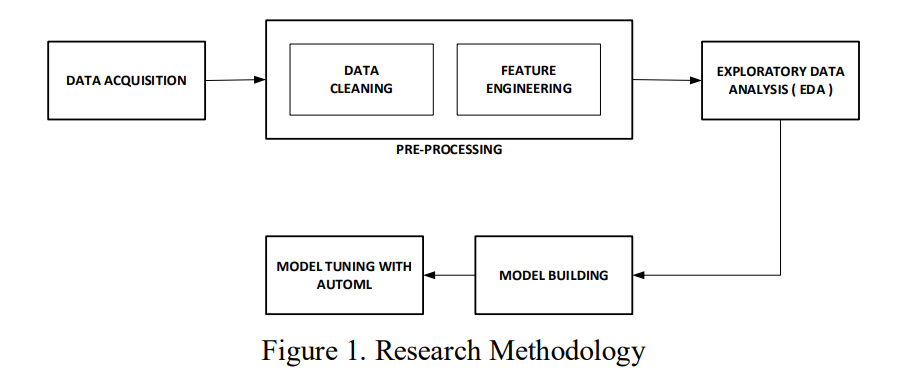
\includegraphics[scale=0.75]{method.png}
\section{ Data Acquisition}
In this study, the dataset came from Muhammet 
Varli's "Laptop Price" repository on the Kaggle 
website [7]. This dataset has 12 columns containing 
up to 1303 rows of data. Each column is a 
specification of a laptop in general, such as the 
brand, CPU, VGA/GPU, the price. Details of this 
"Laptop Price" dataset can be seen in Figure 2.\hfill
\vspace*{1cm}
    \hspace*{-1cm}                                                           
        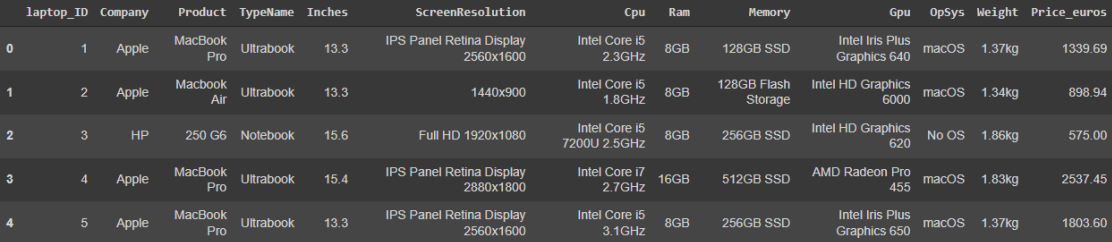
\includegraphics[scale=0.75]{2.png}
\vspace*{0.3cm}
    \hspace*{6cm}                                                           
        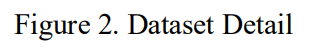
\includegraphics[scale=0.75]{3.png}
\section{Data Cleaning}
Data Cleaning increases the usability of the 
dataset used. For example, in this study, all 
column names in the dataset will be changed to 
lowercase. The syntax for performing Data Cleaning 
can be seen in Figure 3.\hfill
\vspace*{1cm}
    \hspace*{0cm}                                                           
        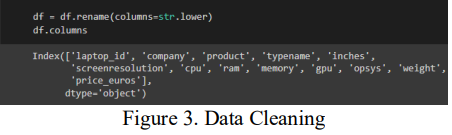
\includegraphics[scale=1.5]{4.png}
\section{Basic data exploration}
After loading the dataset via Pandas, we can see a
list of laptops and specsthat are associated with each 
laptop. Looking at the dataset, we can see that some 
columns such asScreen Resolution and CPU have 
alphanumericdata while other features consist of
purely numerical or alphabetical values. These data
would need to be filtered and engineered later. To 
avoid any complications and error-prone
predictions, useless features such as “Unamed:0”, 
“Company” and “Product” willbe removed from the
dataset.
\section{ Feature Engineering}
We would now extract and reorganize our data to
better understand the underlying factors that contribute to the price of laptops. If we take a look at 
the Screen Resolution column, there seems to be 
laptops with touchscreen capabilities. Since 
touchscreen laptops are known to be more expensive 
than those without them, a TouchScreen feature 
would beadded to mark laptops with such capabilities.
Feature Engineering serves to create more 
features from existing datasets [10], [11]. In this 
study, the laptop specification column, such as CPU, 
will be broken down into several new columns, 
namely CPU Brand and CPU Clock. The syntax for 
performing Feature Engineering can be seen in 
Figure 4, and the overall results can be seen in Table 
1.\hfill\break\break
\vspace*{0cm}
    \hspace*{-2cm}                                                           
        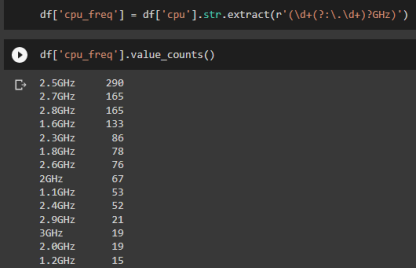
\includegraphics[scale=0.8]{5.png}
\break
\vspace*{0cm}
    \hspace*{4cm}                                                           
        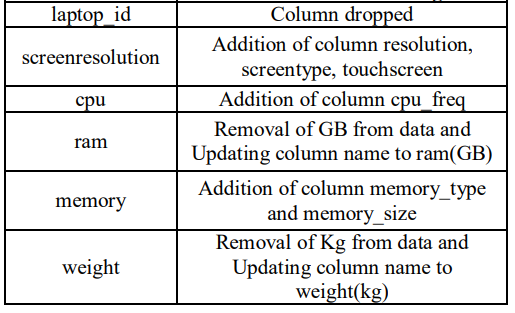
\includegraphics[scale=0.8]{6.png}

\vspace*{0cm}
    \hspace*{5cm}                                                           
        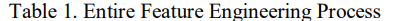
\includegraphics[scale=0.8]{7.png}

\section{Explanatory Data Analysis (EDA)}
Using our feature-engineered dataset, we cannow plot 
graphs and compute tables to visualize how each 
feature relates to the variability of laptop prices.
By using the barplot method imported from
Matplotlib, we can test and verify our hypothesis or 
initial opinions on how some features will affect the
pricing of laptops.
Here’s an illustration of plotting a barplot for the
feature TypeName (type of laptop)\break\break
% \vspace*{2cm}
    % \hspace*{3cm}                                                       
        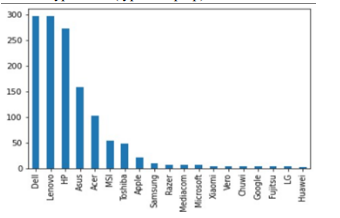
\includegraphics[scale=1.25]{8.png}\break\break\break

% \vspace*{0cm}
    % \hspace*{0cm}                                                           
        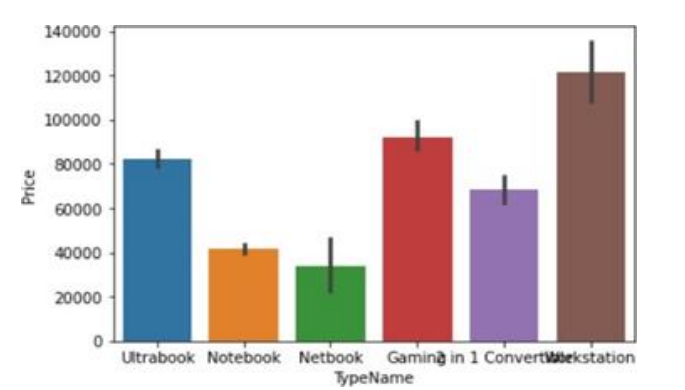
\includegraphics[scale=0.8]{9.png}\break
From the barplot above, we can rectify and conclude that, on average, workstation and gaming laptops have a higher price than other types of laptops.This is to be expected as these types of laptops often have better spec configurations (better CPU, more memory, etc.) to meet the demands of clients in the professional workspace. Notebooks and netbooks have lower prices due to their low- powered configurations. 
Plotting bar graphs on the CPU features shows some interesting results. In general, higher-powered 
processors should be priced higher than lower powered ones. The prices for intel processors 
generally follow this pattern (Xeon > i7>i5>i3) and 
the same principles apply to AMD CPUs as well
(Ryzen > AMD A series> E series).
\hfill
\section{Data Preprocessing}
In this section, we will relabel and convert
categorical features into numerical features. This is 
essential for training our ML models asML models 
only accept numerical values as inputs.
Starting off, we identify features that are non numerical (Object type) and compute their
cardinalities (categories present in each feature).

\section{Dataset Splitting}
The dataset will be split twice before model 
generation into train-testing data. In this study, the 
configuration of the dataset splitting used i.e., 
85 percent of the dataset will be training data, while 15 percent
will be testing data. The dataset splitting process can 
be seen in Figure 6.\hfill\break\break
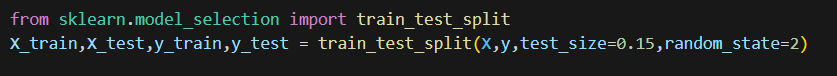
\includegraphics{10.png}
\section{Model Building}
After loading the preprocessed .csv dataset, we 
identify our dependent variable (Price) and allocate 
a separate data frame for the target variable.
Machine Learning is finding patterns in data,and 
one can perform either supervised or unsupervised 
learning. ML tasks include regression, 
classification, forecasting, and clustering.
In this stage of the process, one has to apply
mathematical, computer science, and business
knowledge to train a Machine Learning algorithm 
that will make predictions based on the provided 
data. It is a crucial step that will determine the 
quality and accuracy of future predictions in new 
situations. Additionally, ML algorithms help to 
identify key features with high predictive value.\break
In this study, ten basic regression algorithms 
are generally used to create a machine learning 
model that can predict laptop prices, namely 
\begin{itemize}
    \item Random Forest
    \item Voting Regressor
    \item  XGBoost
    \item Decision Tree
    \item Ridge Regression
    \item Lasso Regression
    \item SVM
    \item Linear Regression
    \item KNN
    \item AdaBoost
\end{itemize}

\section{Website}
Streamlit library is used to build this WebAppUI. 
Streamlit is an open-source \hfill python library that 
makes it easy to create and share, custom web apps 
for machine learning and data science. Result is
shown in following figures,\hfill\break\break
    \centering
    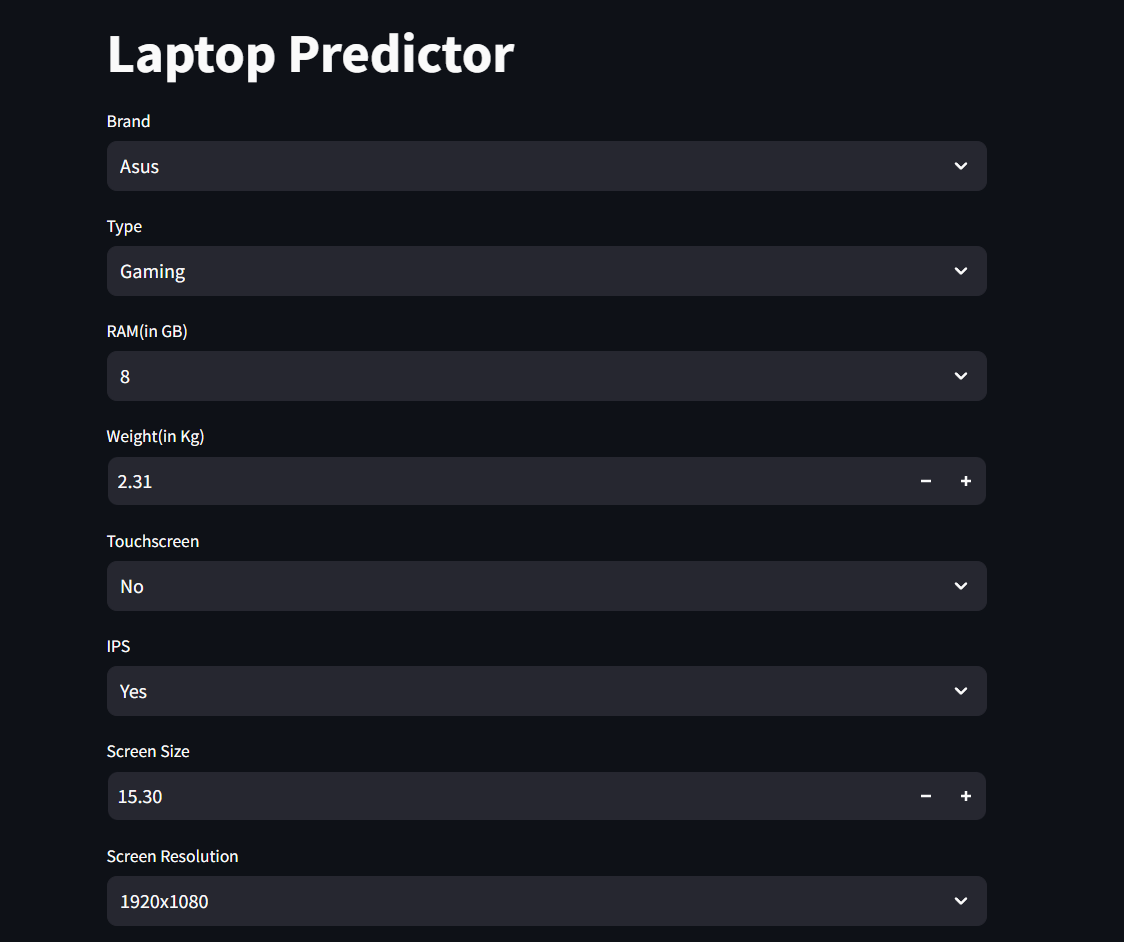
\includegraphics[width=0.5\linewidth]{12.png}
    \break\break
    \centering
    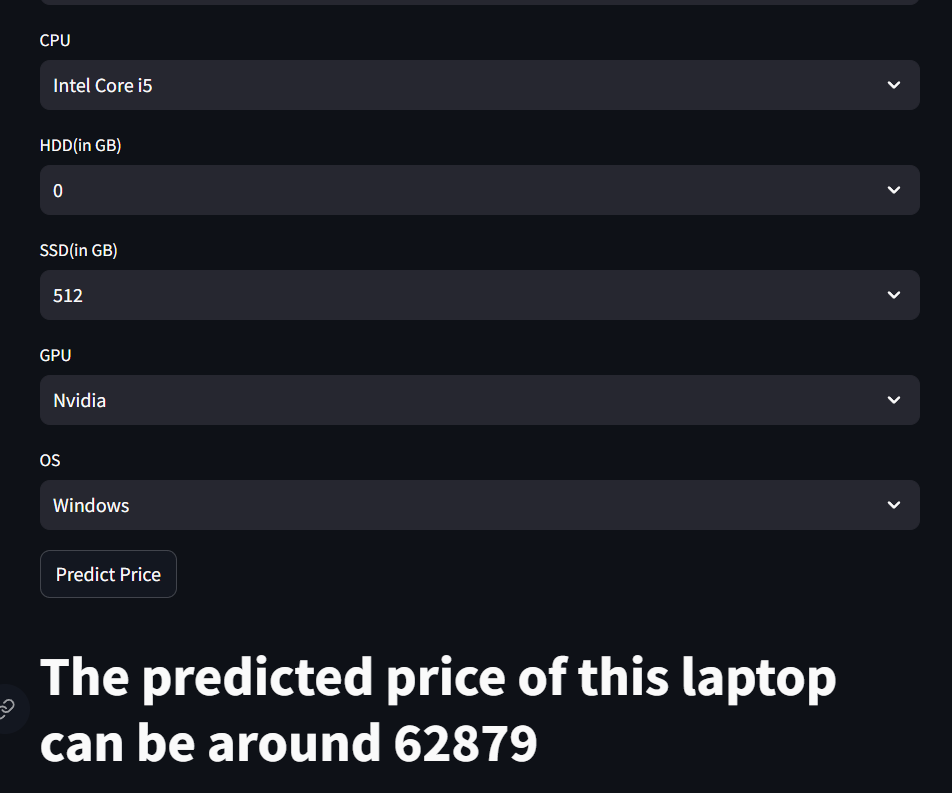
\includegraphics[width=0.5\linewidth]{13.png}

\chapter{Analysis of Proposed Model Performance}
% Content for Analysis section goes here
The Random Forest algorithm is used in building a
model to predict the price of the laptop.
"Random Forest is a classifier that contains a number
of decision trees on various subsets of the given dataset 
and takes the average to improve the predictive 
accuracy of that dataset." Instead of relying on one 
decision tree, the random forest takes the prediction
from each tree and based on the majority votes of
predictions, and it predicts the final output.
The greater number of trees in the forest leads to
higher accuracy and prevents the problem of
overfitting.\hfill\break\break\break
    \vspace{2cm}
    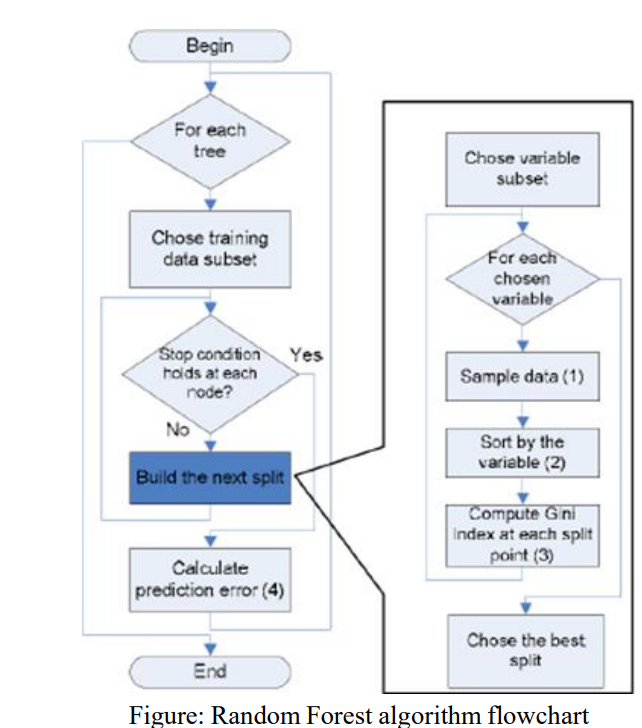
\includegraphics[scale=0.75]{11.png}
\break\break\break
\begin{itemize}
    \item The Working process can be explained in the below
steps
\item Step-1: Select random K data points from the training
set.
\item Step-2: Build the decision trees associated with the
selected data points (Subsets).
\item Step-3: Choose the number N for decision trees that
you want to build.
\item Step-4: Repeat Step 1 and 2.
\item Step-5: For new data points, find the predictions of
each decision tree, and assign thenew data points to 
the category that wins the majority votes.
\end{itemize}
\chapter{Comparison of Performance with other Models}
% Content for Comparison section goes her
\begin{justify}

The comparison is done on the basis of R2 score and MAE.
\break
R2 Score:The R2 score is a value between 0 and 1. A score of 1 indicates that the regression model perfectly predicts the dependent variable, while a score of 0 indicates that the model does not explain any of the variability in the dependent variable.In other words, R2 measures the proportion of the response variable's variance that is captured by the model. It is calculated using the formula:\break\break
% \vspace*{3cm}
    \hspace*{0cm} 
        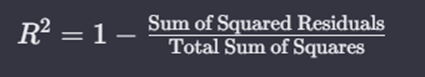
\includegraphics[scale=1.0]{14.png}
\break\break\break
MAE: MAE stands for Mean Absolute Error. It is a metric used to evaluate the performance of a regression model. The Mean Absolute Error measures the average absolute difference between the actual and predicted values. The formula for calculating MAE is as follows:\hfill\break
\begin{figure}
    \centering
    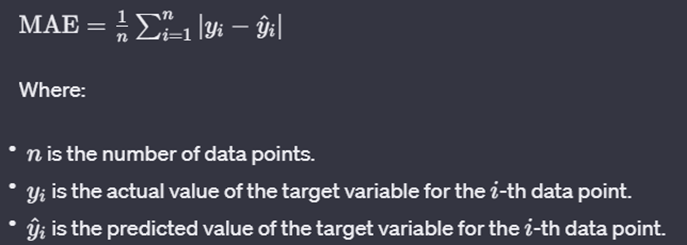
\includegraphics[width=0.5\linewidth]{15.png}
\end{figure}
\end{justify}
\break
\begin{figure}
    \centering
    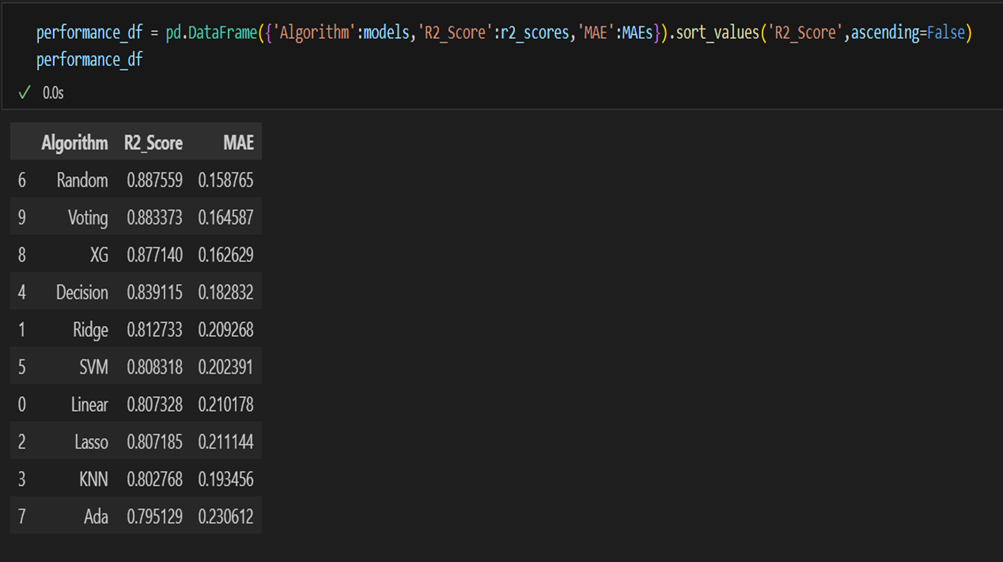
\includegraphics[width=0.7\linewidth]{17.png}
    \caption{Comparison Table}
    \label{fig:enter-label}
\end{figure}
\begin{figure}
    \centering
    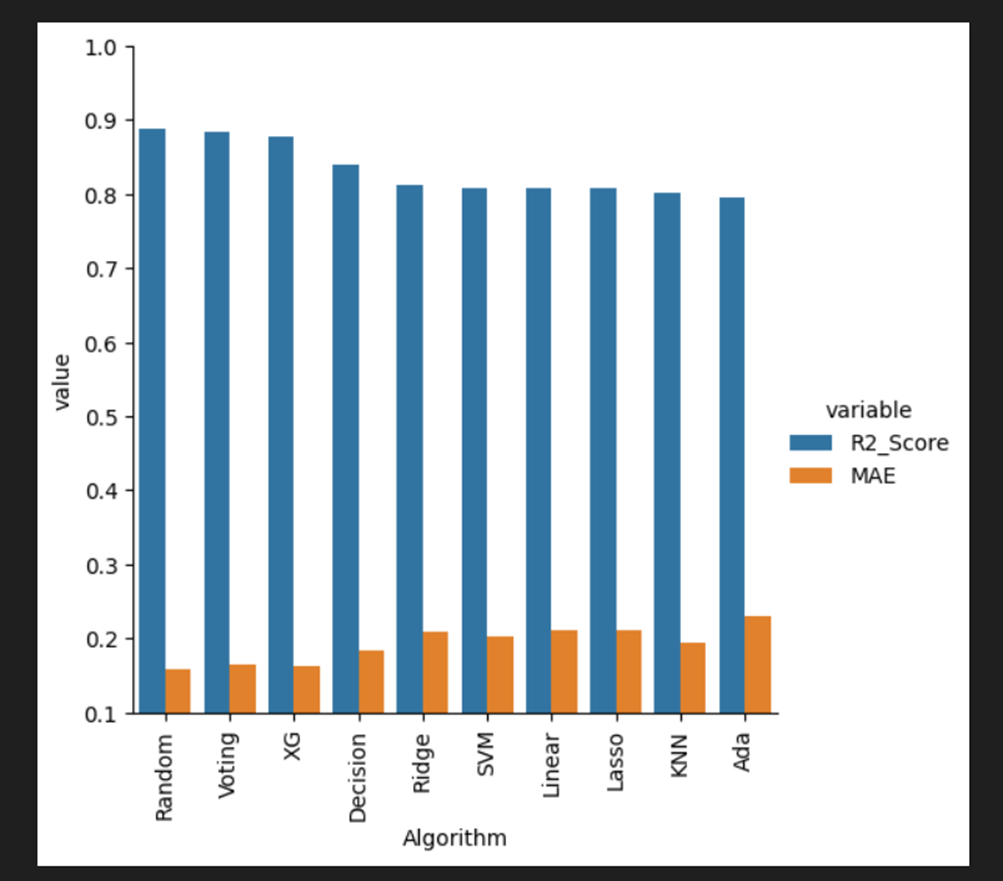
\includegraphics[scale=0.7]{16.png}
    \caption{Plot for comparison}
    \label{fig:enter-label}
\end{figure}

\chapter{Conclusion and Future Work}
% Content for Conclusion and Future Work section goes here
\begin{justify}
Predicting something through the application of machine learning using the Decision Tree algorithm makes it easy for students, especially in determining the choice of laptop specifications that are most desirable for students to meet student needs and in accordance with the purchasing power of students. Students no longer need to look for various sources to find laptop specifications that are needed by students in meeting the needs of students, because the laptop specifications from the results of the machine learning application have provided the most desirable specifications with their prices of laptops. With a model that can predict the price of a laptop, employees can more easily determine the laptop that suits their needs. In this study, the model with the highest R2 value and the lowest MAE is RandomForest, with an R2 value of 88.77 percent and an MAE of 0.15. Therefore, Random Forest can be said
to be better than other predicting Models. The Random Forest model that has been created can also be used to make predictions in real-time using a web-based Machine Learning application.
\end{justify}
% \chapter{Bibliography}
% \bibliographystyle{plain}
% \bibliography{Project}
\begin{flushleft}
    \section{Future Work}
\end{flushleft}
\begin{itemize}
    \item \textbf{Additional Features:}
Explore gathering more data such as specifications, brand reputation, user reviews, or market trends.

\item \textbf{Enhanced Data Quality:}
Improve data quality through robust data cleaning and explore imputation methods for missing values.

\item \textbf{Advanced Models:}
Evaluate more sophisticated models like ensemble methods or deep learning for potentially improved predictions.

\item \textbf{Hyperparameter Tuning:}
Fine-tune hyperparameters more exhaustively to optimize model performance.

\item \textbf{Temporal Analysis:}
Incorporate temporal analysis to account for changes in laptop prices over time.

\item \textbf{Cross-Domain Predictions:}
Adapt the model for predicting prices in related domains like other electronic devices.

\item \textbf{User Interface Development:}
Create a user interface or web app for easier model accessibility.

\item \textbf{Benchmarking:}
Compare your model against other existing models or benchmarks for performance evaluation.

\item \textbf{Interpretability:}
Enhance model interpretability for better understanding and trust.

\item \textbf{Collaboration with Experts:}
Collaborate with industry experts to refine features and improve model accuracy.
\end{itemize}
\end{document}

% \tableofcontents % Prints the main table of contents

%\listoffigures % Prints the list of figures

%\listoftables % Prints the list of tables

%----------------------------------------------------------------------------------------
%	ABBREVIATIONS
%----------------------------------------------------------------------------------------

% \begin{abbreviations}{ll} % Include a list of abbreviations (a table of two columns)

% \textbf{LAH} & \textbf{L}ist \textbf{A}bbreviations \textbf{H}ere\\
% \textbf{WSF} & \textbf{W}hat (it) \textbf{S}tands \textbf{F}or\\

% \end{abbreviations}

%----------------------------------------------------------------------------------------
%	PHYSICAL CONSTANTS/OTHER DEFINITIONS
%----------------------------------------------------------------------------------------

% \begin{constants}{lr@{${}={}$}l} % The list of physical constants is a three column table

% % The \SI{}{} command is provided by the siunitx package, see its documentation for instructions on how to use it

% Speed of Light & $c_{0}$ & \SI{2.99792458e8}{\meter\per\second} (exact)\\
% %Constant Name & $Symbol$ & $Constant Value$ with units\\

% \end{constants}

%----------------------------------------------------------------------------------------
%	SYMBOLS
%----------------------------------------------------------------------------------------

% \begin{symbols}{lll} % Include a list of Symbols (a three column table)

% $a$ & distance & \si{\meter} \\
% $P$ & power & \si{\watt} (\si{\joule\per\second}) \\
% %Symbol & Name & Unit \\

% \addlinespace % Gap to separate the Roman symbols from the Greek

% $\omega$ & angular frequency & \si{\radian} \\

% \end{symbols}

%----------------------------------------------------------------------------------------
%	DEDICATION
%----------------------------------------------------------------------------------------

% \dedicatory{For/Dedicated to/To my\ldots} 

%----------------------------------------------------------------------------------------
%	THESIS CONTENT - CHAPTERS
%----------------------------------------------------------------------------------------

% \mainmatter % Begin numeric (1,2,3...) page numbering

% \pagestyle{thesis} % Return the page headers back to the "thesis" style

% Include the chapters of the thesis as separate files from the Chapters folder
% Uncomment the lines as you write the chapters

% \include{Chapters/Chapter1}
%\include{Chapters/Chapter2} 
%\include{Chapters/Chapter3}
%\include{Chapters/Chapter4} 
%\include{Chapters/Chapter5} 

%----------------------------------------------------------------------------------------
%	THESIS CONTENT - APPENDICES
%----------------------------------------------------------------------------------------

% \appendix % Cue to tell LaTeX that the following "chapters" are Appendices

% Include the appendices of the thesis as separate files from the Appendices folder
% Uncomment the lines as you write the Appendices

% \include{Appendices/AppendixA}
%\include{Appendices/AppendixB}
%\include{Appendices/AppendixC}

%----------------------------------------------------------------------------------------
%	BIBLIOGRAPHY
%----------------------------------------------------------------------------------------

% \printbibliography[heading=bibintoc]

%----------------------------------------------------------------------------------------

% \end{document}  
